\subsection{Serviceorientierte Architektur (SOA)}

\textbf{Service (Dienst)}

Angebot einer Geschäftsprozess oder IT-Dienstleistung, Zugriff über eine klar geregelte Schnittstelle (Interface)

\subsubsection{Grundprinzipien}

\begin{itemize}
    \item \textcolor{blue}{Geschäftsrelevante Services} bildet meist eine Teilfunktion eines Geschäftsprozesses
    \item \textcolor{blue}{Service Kontrakt: Service Level Agreement (SLA)} Inhalt/Zweck der Leistungserbringung, QoS (Quality of Service wie z.B. Verfügbarkeit, Performanz usw.), Zugriff (Authentisierung, Autorisierung), Support, Kosten, Sanktionen
    \item \textcolor{blue}{Service Auffindbarkeit} Service ist in einem Verzeichnis registriert
    \item \textcolor{blue}{Servicekomposition} Mehrere Services können z.B. im Rahmen eines Geschäftsprozesses im Workflow komponiert werden
\end{itemize}

\subsubsection{Service Lifecycle}

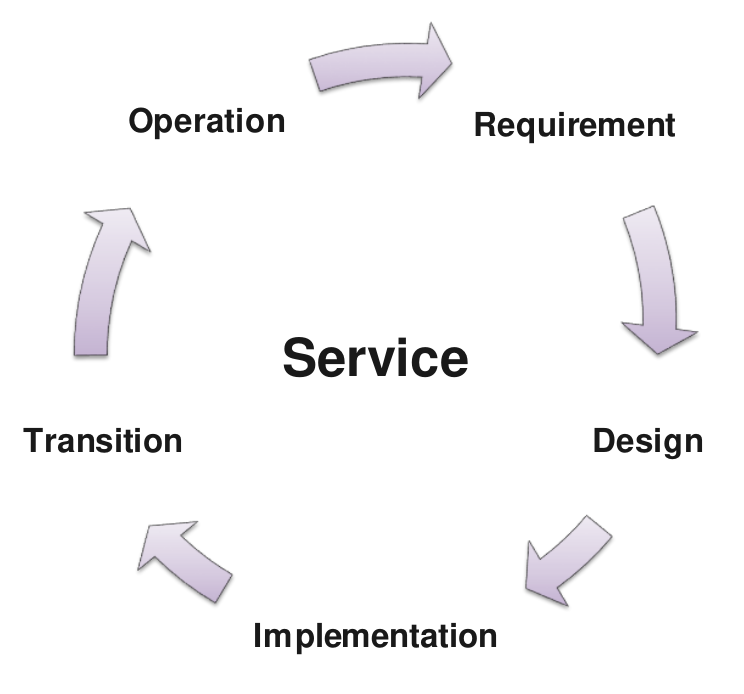
\includegraphics[width=0.6\linewidth]{soa-service-lifecycle.png}

\begin{enumerate}
    \item \textcolor{blue}{Requirements} Aufnahme der Anforderungen
    und Abstimmung mit den Stakeholdern
    \item \textcolor{blue}{Design} Serviceengineer beschreibt API, Funktionalität, Konfigurierbarkeit usw. und legt das SLA mit den Konsumenten fest.
    \item \textcolor{blue}{Implementation} Softwareentwickler implementiert den Service
    \item \textcolor{blue}{Transition} (Einführung) Installation, Publikation im Dienstverzeichnis, sowie Information bzw. Instruktion für betreffende Stakeholder
    \item \textcolor{blue}{Operation} Nutzung mit fortlaufendem Monitoring $\rightarrow$ neue Anforderungen zur Optimierung oder Erweiterung
\end{enumerate}

\subsubsection{Fundamentales SOA-Dreieck}

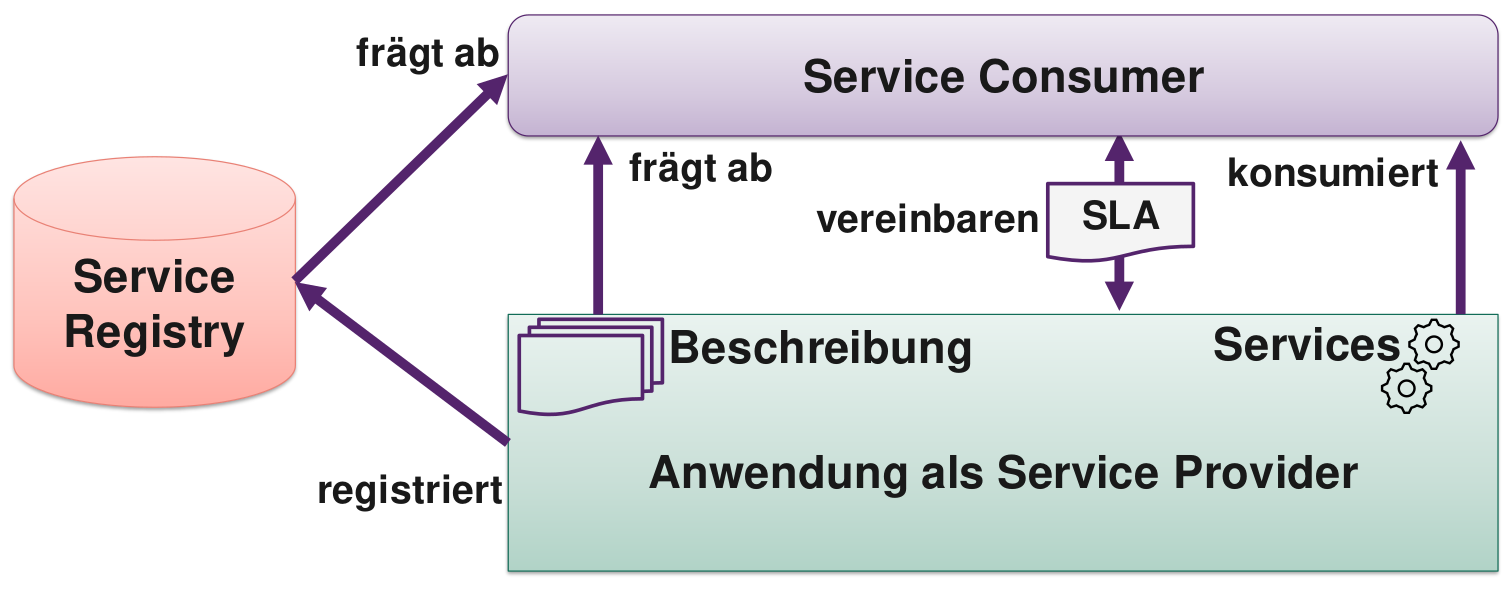
\includegraphics[width=\linewidth]{soa-soa-dreieck.png}

\columnbreak
\subsubsection{Service Modellierung (SoaML)}

\textbf{Service-oriented architecture Modeling Language (SoaML)}

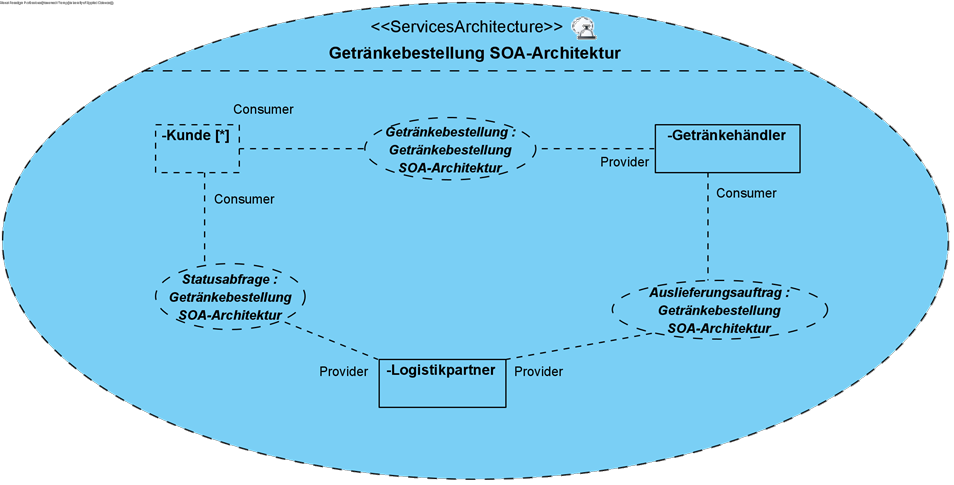
\includegraphics[width=\linewidth]{soa-modeling.png} \\

Beispiel

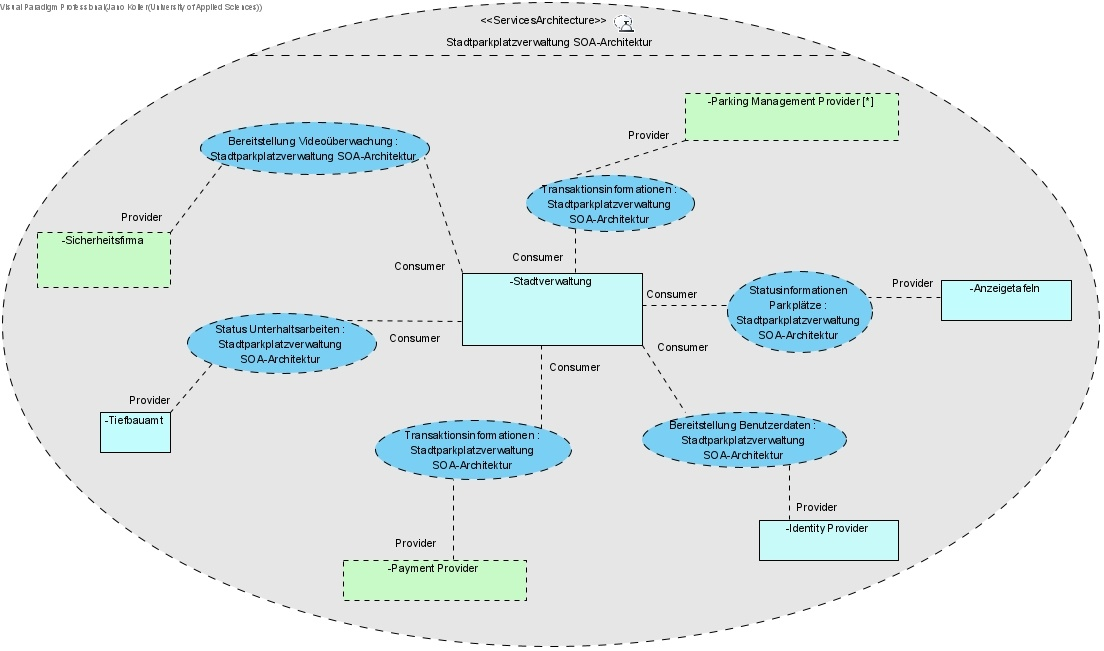
\includegraphics[width=\linewidth]{soa-example.png} \\

\textbf{Sequenzdiagramm}

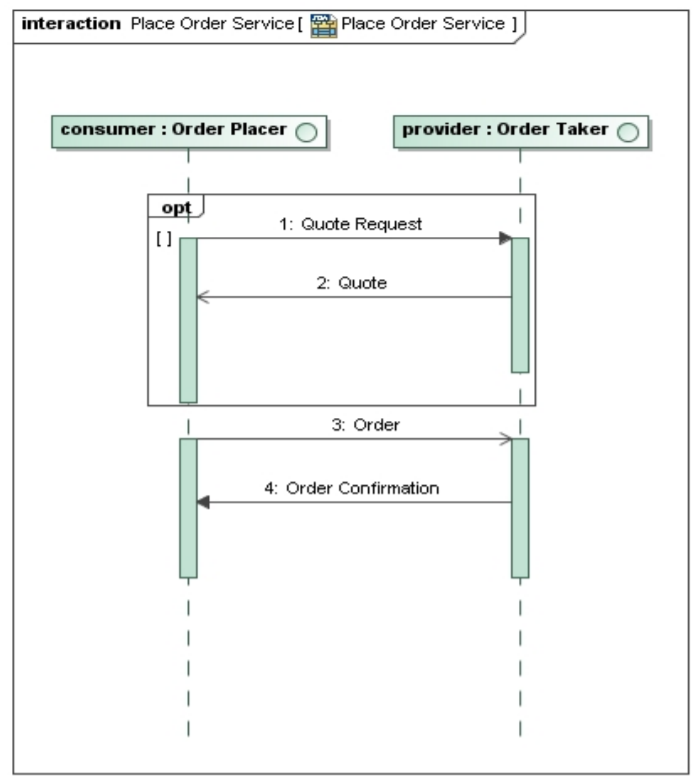
\includegraphics[width=0.7\linewidth]{soa-sequence-diagram.png}

\columnbreak
\subsubsection{Synchrone Web Services}

\textbf{SOAP}

Simple Object Access Protocol, zustandsbehaftet, ruft Funktionen bzw. Methoden auf, mit der WSDL (Web Service Description Language) werden Schnittstellen beschrieben, funktioniert auf Anwendungsebene folgendermassen

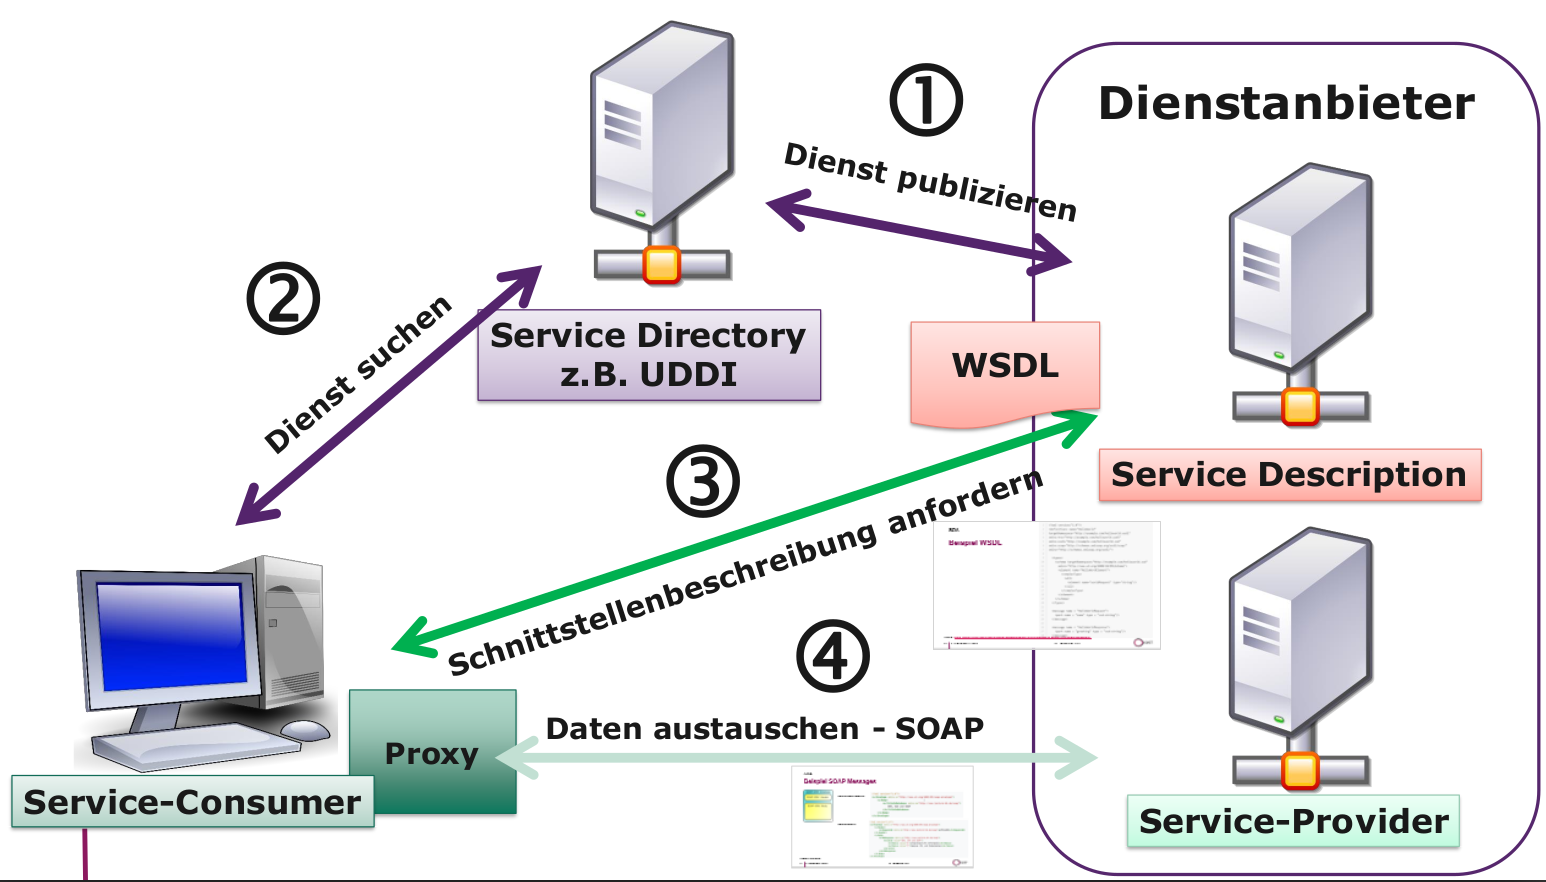
\includegraphics[width=\linewidth]{soa-soap.png}

\begin{enumerate}
    \item Service-Provider publiziert SOAP-Dienst beim Service Directory, basiert bspw. auf UDDI (universal Description, Discovery and Integration)
    \item Service-Consumer sucht in Service Directory nach dem Service und erhält URI für Schnittstellenbeschreibung
    \item Mit der aufgerufenen WSDL-Beschreibung kann Consumer-Runtime den Proxy automatisch erstellen
    \item Proxy fungiert als Adapter, um die Methoden des SOAP-Services ansprechen zu können
\end{enumerate}
\vspace{10pt}
\textbf{REST}

Representational State Transfer, ressourcenorientiert, zustandslos, verwendet HTTP-Befehle, Payload ist meist JSON, kann aber auch XML oder anders Format sein, hat keine standardisierte Schnittstellenbeschreibung


\begin{itemize}
    \item \textcolor{blue}{GET} Ressource(n) [z.B. Kunde(n)] anfordern
    \item \textcolor{blue}{POST} einfügen einer Ressource (z.B. Kunde), senden einer Message
    \item \textcolor{blue}{PUT} ändern einer Ressource
    \item \textcolor{blue}{MERGE} Teil einer Ressource ändern
    \item \textcolor{blue}{DELETE} löschen einer Ressource
\end{itemize}
\vspace{10pt}
\textbf{OData}

REST-basierter flexibler Datendienst, basiert auf Metadaten, Bietet Datenressourcen und Funktionen an, Payload ist JSON oder AtomPub (XML) \\

\textbf{GraphQL}

Query-Sprache, erlaubt gezielte Bearbeitung von Daten, Schema Definition Language, kann Daten aus mehreren Ressourcen zusammennehmen, Arbeitet mit HTTP - POST

\columnbreak
\subsubsection{Asynchrone Kommunikation}

Kommunikation mittels Nachrichten (Messages), Sender und Empfänger sind zeitlich entkoppelt, ermöglicht hohe Parallelität mit geringen Ressourcenverbrauch, \textcolor{blue}{Kommunikation mittels Message Oriented Middleware (MOM)} \\

Vorteile

\begin{itemize}
    \item lose Kopplung zwischen Applikationen
    \item hohe Fehlertoleranz
    \item geringer Ressourcenverbrauch
    \item schnelle parallele Verarbeitung
    \item dynamische Skalierung
    \item hohe Flexibilität bei Änderungen
\end{itemize}

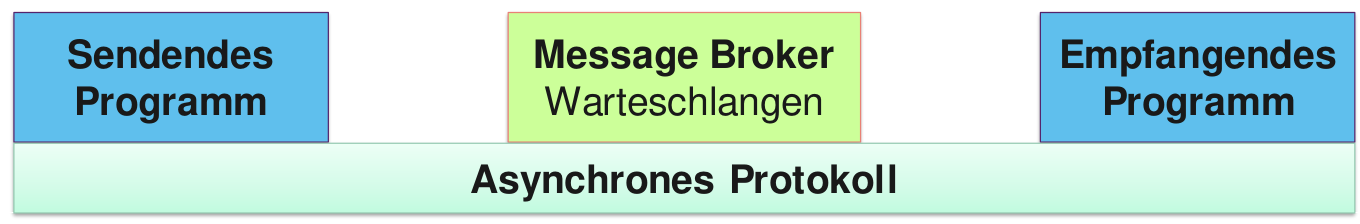
\includegraphics[width=\linewidth]{soa-mom.png}

\textbf{Protokolle}

\textcolor{blue}{AMQP} Advanced Message Queuing Protocol ist ein standardisiertes asynchrones Message-Protokoll zur Kommunikation zwischen Client und Message Broker sowie zwischen unterschiedlichen Message Brokern.

\textcolor{blue}{MQTT} für IoT \\

\textbf{Message Broker}

verwaltet diverse Queues. Er vermittelt und speichert die erhaltenen Nachrichten un untersützt unterschiedliche Kommunikationsmuster.

\textcolor{blue}{RabbitMQ} Open Source, Message Store, Message Passing (One-Way) oder Request-Reply

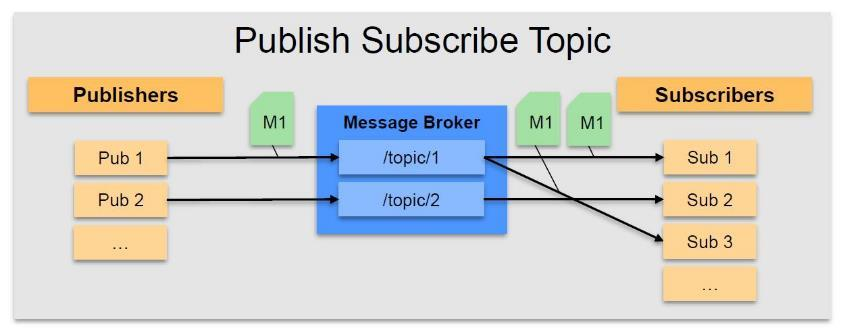
\includegraphics[width=0.8\linewidth]{soa-rabbitmq-1.png}

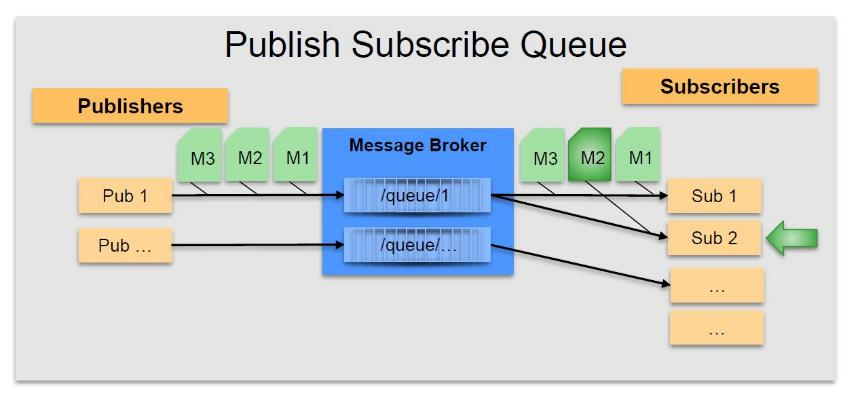
\includegraphics[width=0.8\linewidth]{soa-rabbitmq-2.png} \\

Publish
\begin{lstlisting}
asyncapi: 2.2.0
info:
  title: Hello world application
  version: '0.1.0'
channels:
  hello:
    publish:
      message:
        payload:
          type: string
          pattern: '^hello .+$'
\end{lstlisting}
\vspace{10pt}
\columnbreak
Subscribe
\begin{lstlisting}
asyncapi: 2.2.0
info:
  title: Example
  version: 0.1.0
channels:
  user/signedup:
    subscribe:
      message:
        description: An event describing
        payload:
          type: object
          additionalProperties: false
          properties:
            fullName:
              type: string
            email:
              type: string
              format: email
            age:
              type: integer
              minimum: 18
\end{lstlisting}

\subsubsection{Elektronische Nachricht}

\textbf{1. Ebene: Semantik}

Inhaltliche Bedeutung (im Anwendungskontext)

\begin{itemize}
    \item \textcolor{blue}{Nachrichtentyp} Bsp. Offer, Order, Invoice
    \item \textcolor{blue}{Basisstruktur} Bedeutung einzelner Felder, Datentyp, Codetabellen, gültige Werte
\end{itemize}

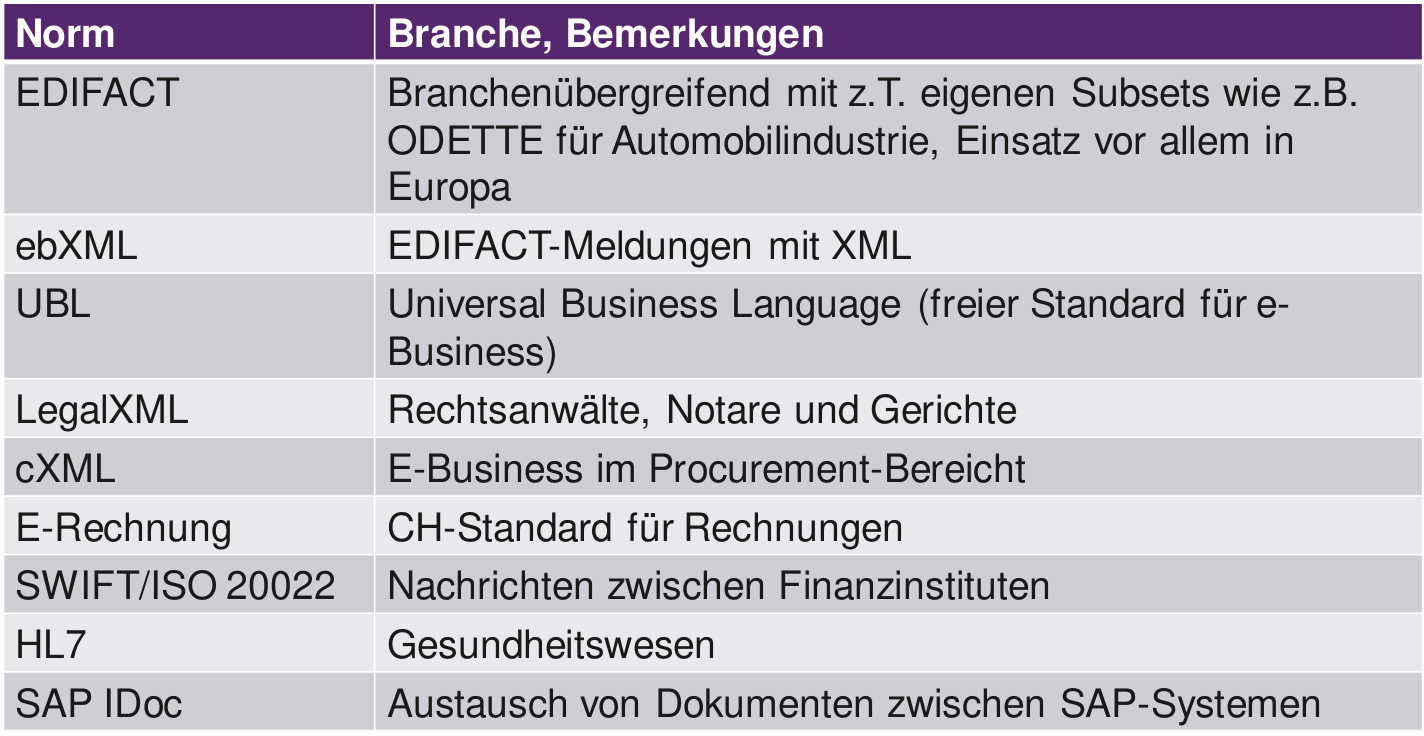
\includegraphics[width=\linewidth]{soa-semantic.png} \\


\textbf{2. Ebene: Format}

Technischer Aufbau/Struktur einer Nachricht

\begin{itemize}
    \item \textcolor{blue}{CSV} Comma Separated Values, kompakt, plattformspezifisch
    \item \textcolor{blue}{EDI} Electronic Data Interchange, klassische» EDIFACT-Meldungen, E-Business, branchenübergreifend
    \item \textcolor{blue}{XML} Extended Markup Language, gibt bis zu 50 \% Overhead, plattformunabhängig, HTML für E-Mail
    \item \textcolor{blue}{JSON} JavaScript Object Notation, kompakter als XML, bei RESTful-Services beliebt
\end{itemize}
\vspace{10pt}
\textbf{3. Ebene: Codierung}

Definiert die verwendete Codetabelle für die Bitfolgen je Zeichen, Bitfolge für die Festlegung der Zeichen

\begin{itemize}
    \item \textcolor{blue}{ASCII} ANSI-Standard
    \item \textcolor{blue}{EBCDIC} IBM-Standard
    \item \textcolor{blue}{Unicode} internationaler Standard, jedes Zeichen in der Welt hat eine fixe Bitkombination: 8 / 16 oder 32 bit, UTF-8
\end{itemize}

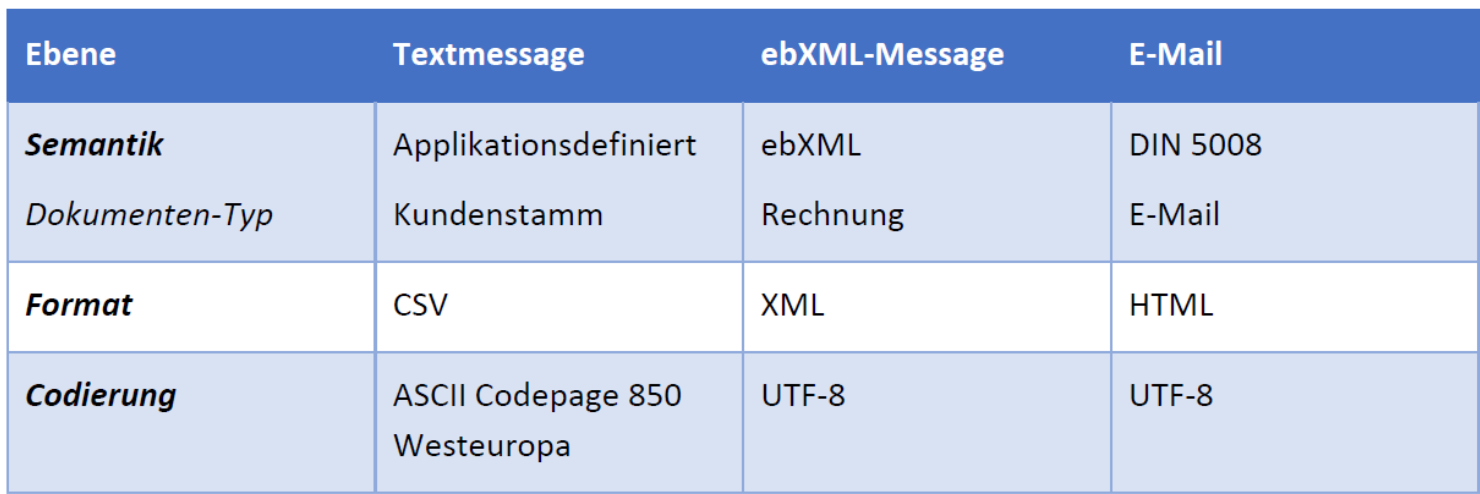
\includegraphics[width=\linewidth]{soa-message-example.png}

\subsubsection{IT-Sicherheit}

\textbf{Schutzziele}

\begin{itemize}
    \item \textcolor{blue}{Vertraulichkeit} Unbefugter Informationsgewinn
    \item \textcolor{blue}{Integrität} Unbefugte Modifikation (Änderung) von Daten bzw. Funktionen
    \item \textcolor{blue}{Verfügbarkeit} Unbefugte Beeinträchtigung der Funktionalität bzw. Verfügbarkeit
    \item \textcolor{blue}{Nachweisbarkeit} Nachvollziehbarkeit bzw. Nichtabstreitbarkeit einer Handlung
\end{itemize}
\vspace{10pt}
\textbf{Zugriffssicherheit}

Schutz vor unerlaubter Nutzung

SSO (Single Sign On) Lösungen
\begin{itemize}
    \item \textcolor{blue}{SAML} Security Assertion Markup Language
    \item \textcolor{blue}{OAuth 2.0} für Webservices, Token orientiert
\end{itemize}
\vspace{10pt}
\textbf{Messagesicherheit}

End-zu-End Verschlüsselung

\begin{itemize}
    \item \textcolor{blue}{XML-Message Security} XML Encryption (Verschlüsselung der XML-Nachricht), XML Signature (Digitales signieren einer XML-Nachricht)
    \item \textcolor{blue}{E-Mail Security} S-/MIME, PGP
\end{itemize}


\subsubsection{API Entwicklung}

\begin{enumerate}
    \item \textcolor{blue}{Service Requirements} Anforderungen an den Service im Detail festlegen
    \item \textcolor{blue}{Design} Entwickler entwirft einzusetzende Technologien, Funktionsumfang, Inhalte und Integration der API
    \item \textcolor{blue}{Mocking (Prototype)} Entwickler erstellt mit dem Spezifikationen einen Prototypen
    \item \textcolor{blue}{Validate} Mit dem Mockup-Service validiert Entwickler die Schnittstelle mit den Stakeholdern
    \item \textcolor{blue}{Build} Entwicklung der API und Integration mit dem Backend
    \item \textcolor{blue}{Document} Dokumentation der Verwendung der API
    \item \textcolor{blue}{Test} Nachweis für die korrekte Funktionalität und QoS
    \item \textcolor{blue}{Deploy and Publish} Verteilung der API auf Zielplattform und Publikation im Service Directory
    \item \textcolor{blue}{Monitor} Überwachung der Nutzung der API
\end{enumerate}

\subsubsection{API Management}

\textbf{Funktionen}

\begin{itemize}
    \item \textcolor{blue}{API Lifecycle Management} Sicherstellung der Konsistenz zwischen verschiedenen Versionen
    \item \textcolor{blue}{API-Governance (Einhalten von Policies [Richtlinien])}
    \item \textcolor{blue}{API-Sicherheit} SSL Offloading, Authentisierung zum Schutz der API vor Missbrauch
    \item \textcolor{blue}{Automatisiertes API-Deployment und Publishing} anhand Policies
    \item \textcolor{blue}{API-Gateway mit Load-Balancing und Fault-Tolerance} Sicherstellung einer optimalen Performance durch Caching, Skalierung, Load-Balancing und Fehlertoleranz
    \item \textcolor{blue}{API-Monitoring und Analytics} Monitoring und automatisches Logging für die Überwachung
\end{itemize}

\columnbreak
\subsubsection{Prüfungsfragen}

\begin{itemize}
    \item Was ist das Hauptmerkmal von SOA? \\
    \textcolor{blue}{Bereitstellung von unterschiedlichen
    Services}
    \item Welches sind die drei Schnittstellen eines Service? Erläutern Sie stichwortartig deren Funktion \\
    \textcolor{blue}{Control API, API, und Point of Observation}
    \item Welches sind die fünf Prozessschritte des Service-Lifecycle? \\
    \textcolor{blue}{Requirement, Design, Implementation, Transition, Operation}
    \item Zeichnen Sie das fundamentale SOA-Dreieck mit dessen Komponenten und Interaktionen auf \\
    \textcolor{blue}{Siehe 2.2 SOA-Dreieck}
    \item Welcher Diagrammtyp von SoaML eignet sich für die Kommunikation der Serviceübersicht? \\
    \textcolor{blue}{Service Architecture Diagram}
    \item Zeichnen Sie den Protokollstack einer SOAP-Kommunikation auf \\
    \textcolor{blue}{Envelope (defines message structure), set of encoding rules,     convention for RPC and responses}
    \item Was ist der Vorteil von GraphQL gegenüber REST? \\
    \textcolor{blue}{GraphQL fragt, im Gegensatz zu REST, dynamisch nur die benötigten Objekte und Attribute ab. Serverseitige Applikation wird wie eine Datenbank behandelt.}
    \item Welche Kommunikationsmuster unterstützt ein Message Broker? \\
    \textcolor{blue}{Message Passing, Request-Reply, Publish-Subscribe Topic, Publish-Subscribe FI-FO}
    \item Welche Themen definiert UBL? \\
    \textcolor{red}{Antwort}
    \item Welches Autorisierungsprotokoll würden Sie für einen RESTful-Service einsetzen? \\
    \textcolor{blue}{OAuth 2.0}
    \item Wozu dient XML Signature? \\
    \textcolor{blue}{Damit man sicher sein kann, von wem die Nachricht stammt}
\end{itemize}

